%
% diagrama del preprocesamiento
%
\shorthandoff{<}
\shorthandoff{>}
\tikzsetnextfilename{figures/preprocesamiento/preprocesamiento}
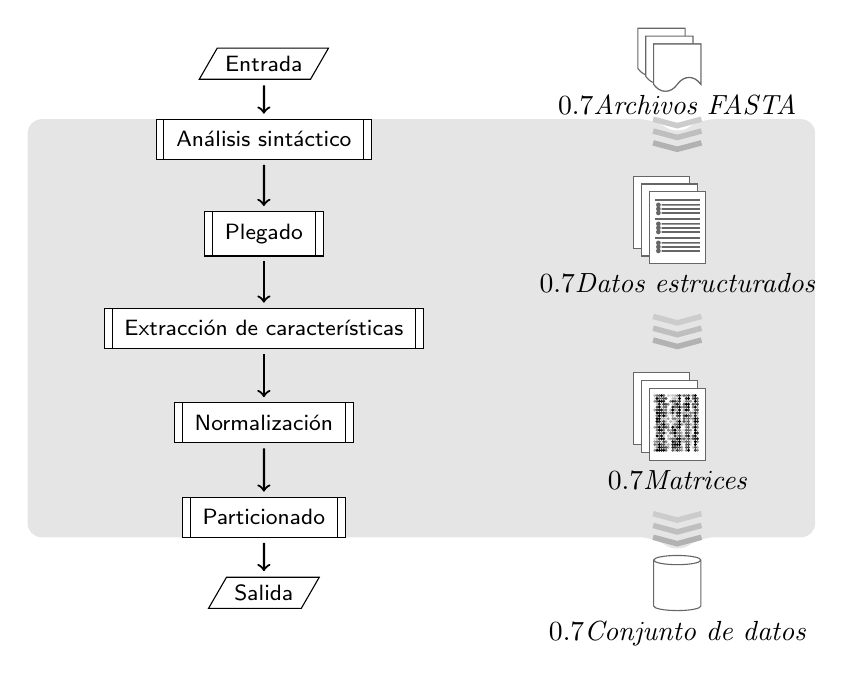
\begin{tikzpicture}[
    %    shorten >=1pt,     % acortar la linea en 1pt al final
    %    shorten <=1pt,     % acortar la linea en 1pt al principio
    %    - stealth,         % estilo de flecha al final (manual pgf p~210)
    font=\footnotesize\sffamily,
    %every label/.style={label distance=4}
  ]
  \usetikzlibrary{
    calc,
    positioning,
    shapes.geometric,
    shapes.symbols,
    shapes.misc,
    shapes.multipart
  }
  %%%%%%%%%%%%%%%%%%%%%%%%%%%%%%%%%%%%%%%%%%%%%%%%%%%%%%%%%%%%%%%%%%%%%%%%
  \tikzstyle{dato}=[
    prefix after command= {\pgfextra{\tikzset{
          every label/.append style={
            font=\relscale{0.7}\itshape,
    }}}}
  ];
  \tikzstyle{archivo}=[
    draw=black!60,
    tape,
    tape bend top=none,
    minimum width=0.6cm,
    minimum height=0.6cm,
    fill=white,
    dato
  ];
  \tikzstyle{archivos}=[
    archivo,
    append after command={\pgfextra{
        \coordinate [] (cen) at ($(\tikzlastnode.center)$);
	\node [archivo] at ($(cen)+(-0.2,0.2)$) {};
	\node [archivo] at ($(cen)+(-0.1,0.1)$) {};
	\node [archivo] at (cen) {};
    }},
  ];
  \tikzstyle{io}=[
    draw,
    trapezium,
    trapezium left angle=60,
    trapezium right angle=120,
    minimum width=1cm,
    inner sep=0.1cm,
  ];
  \tikzstyle{tarea}=[
    rectangle,
    minimum width=1cm,
    inner ysep=0.15cm,
    inner xsep=0.25cm,
    append after command={\pgfextra{
        \coordinate [] (NW) at ($(\tikzlastnode.north west)$);
        \coordinate [] (SE) at ($(\tikzlastnode.south east)$);
        \coordinate [] (A) at ($(\tikzlastnode.north west)+(0.1,0)$);
        \coordinate [] (B) at ($(\tikzlastnode.south west)+(0.1,0)$);
        \coordinate [] (C) at ($(\tikzlastnode.north east)-(0.1,0)$);
        \coordinate [] (D) at ($(\tikzlastnode.south east)-(0.1,0)$);
        \draw[fill=white] (NW) rectangle (SE);
        \draw (A) -- (B);
        \draw (C) -- (D);
    }},
  ];
  \tikzstyle{estruct}=[
    dato,
    minimum width=0.7cm,
    minimum height=0.9cm,
    append after command={\pgfextra{
        \coordinate [] (nw) at ($(\tikzlastnode.north west)$);
        \coordinate [] (se) at ($(\tikzlastnode.south east)$);
        \coordinate [] (ne) at ($(\tikzlastnode.north east)$);
        \coordinate [] (sw) at ($(\tikzlastnode.south west)$);
        \coordinate [] (inw) at ($(nw)!0.1!(se)$);
        \coordinate [] (ine) at ($(ne)!0.1!(sw)$);
        \coordinate [] (isw) at ($(sw)!0.1!(ne)$);
        \coordinate [] (ise) at ($(se)!0.1!(nw)$);
        \coordinate [] (mnw) at ($(inw)!0.08!(ine)$);
        \coordinate [] (msw) at ($(isw)!0.08!(ise)$);
        \coordinate [] (lnw) at ($(inw)!0.15!(ine)$);
        \coordinate [] (lsw) at ($(isw)!0.15!(ise)$);
        %
        \pgfmathsetmacro{\cr}{0.03}
	\draw[black!60,fill=white] ($(sw)+(-0.2,0.2)$) rectangle ($(ne)+(-0.2,0.2)$);
	\draw[black!60,fill=white] ($(sw)+(-0.1,0.1)$) rectangle ($(ne)+(-0.1,0.1)$);
        \draw[black!60,fill=white] (sw) rectangle (ne);
        \fill[black!60,] (inw) rectangle ($(ine)!0.04!(ise)$);
        \fill[black!60,] ($(mnw)!0.10!(msw)$) circle [radius=\cr] 
        ($(mnw)!0.17!(msw)$) circle [radius=\cr]
        ($(mnw)!0.24!(msw)$) circle [radius=\cr];
        \fill[black!60,] ($(lnw)!0.085!(lsw)$) rectangle ($(ine)!0.115!(ise)$) 
        ($(lnw)!0.155!(lsw)$) rectangle ($(ine)!0.185!(ise)$)
        ($(lnw)!0.225!(lsw)$) rectangle ($(ine)!0.255!(ise)$);
        %
        \fill[black!60,] ($(inw)!0.33!(isw)$) rectangle ($(ine)!0.37!(ise)$);
        \fill[black!60,] ($(mnw)!0.43!(msw)$) circle [radius=\cr] 
        ($(mnw)!0.5!(msw)$) circle [radius=\cr]
        ($(mnw)!0.57!(msw)$) circle [radius=\cr];
        \fill[black!60,] ($(lnw)!0.415!(lsw)$) rectangle ($(ine)!0.445!(ise)$) 
        ($(lnw)!0.485!(lsw)$) rectangle ($(ine)!0.515!(ise)$)
        ($(lnw)!0.555!(lsw)$) rectangle ($(ine)!0.585!(ise)$);
        %
        \fill[black!60,] ($(inw)!0.66!(isw)$) rectangle ($(ine)!0.7!(ise)$);
        \fill[black!60,] ($(mnw)!0.76!(msw)$) circle [radius=\cr] 
        ($(mnw)!0.83!(msw)$) circle [radius=\cr]
        ($(mnw)!0.90!(msw)$) circle [radius=\cr];
        \fill[black!60,,shift={(0,-1)}] ($(lnw)!0.745!(lsw)$) rectangle ($(ine)!0.775!(ise)$) 
        ($(lnw)!0.815!(lsw)$) rectangle ($(ine)!0.845!(ise)$)
        ($(lnw)!0.885!(lsw)$) rectangle ($(ine)!0.915!(ise)$);
    }},
  ];
  \tikzstyle{matriz}=[
    minimum width=0.7cm,
    minimum height=0.9cm,
    dato,
    append after command={\pgfextra{
        \coordinate [] (nw) at ($(\tikzlastnode.north west)$);
        \coordinate [] (se) at ($(\tikzlastnode.south east)$);
        \coordinate [] (ne) at ($(\tikzlastnode.north east)$);
        \coordinate [] (sw) at ($(\tikzlastnode.south west)$);
        \coordinate (inw) at ($(nw)!0.1!(se)$);
        \coordinate (ine) at ($(ne)!0.1!(sw)$);
        \coordinate (isw) at ($(sw)!0.1!(ne)$);
        \coordinate (ise) at ($(se)!0.1!(nw)$);
	\draw [black!60,fill=white] ($(sw)+(-0.2,0.2)$) rectangle ($(ne)+(-0.2,0.2)$);
	\draw [black!60,fill=white] ($(sw)+(-0.1,0.1)$) rectangle ($(ne)+(-0.1,0.1)$);
	\draw [black!60,fill=white] (sw) rectangle (ne);
        \pgfmathsetseed{3};
	\foreach \x in {0.0,0.05,...,1} {
	  \coordinate (TOP) at ($(inw)!\x!(ine)$);
	  \coordinate (BOT) at ($(isw)!\x!(ise)$);	
	  \pgfmathsetmacro{\co}{rnd};	
	  \foreach \y in {0.0,0.05,...,1} {
	    \pgfmathsetmacro{\io}{0.5*rand};	
            \fill[black,opacity=\co+\io] ($(TOP)!\y!(BOT)$) circle [radius=0.02];
          }
        }
    }},
  ];
  \tikzstyle{datos}=[
    draw=black!60,
    dato,
    cylinder,
    shape border rotate=90,
    minimum width=0.6cm,
    minimum height=0.7cm,
    %text width=1,
    fill=white,
    shape aspect=.5,
    align=center,
  ];
  \tikzstyle{modelo}=[
    % fill=white,
    minimum width=0.7cm,
    minimum height=0.7cm,
    dato,
    append after command={\pgfextra{
        \coordinate [] (nw) at ($(\tikzlastnode.north west)$);
        \coordinate [] (se) at ($(\tikzlastnode.south east)$);
        \coordinate [] (ne) at ($(\tikzlastnode.north east)$);
        \coordinate [] (sw) at ($(\tikzlastnode.south west)$);
        \coordinate (inw) at ($(nw)!0.1!(se)$);
        \coordinate (ine) at ($(ne)!0.1!(sw)$);
        \coordinate (isw) at ($(sw)!0.1!(ne)$);
        \coordinate (ise) at ($(se)!0.1!(nw)$);
        \coordinate (vnw) at ($(nw)!0.03!(sw)$);
        \coordinate (vne) at ($(ne)!0.03!(se)$);
        \coordinate (vsw) at ($(sw)!0.03!(nw)$);
        \coordinate (vse) at ($(se)!0.03!(ne)$);
        \coordinate (hnw) at ($(nw)!0.03!(ne)$);
        \coordinate (hne) at ($(ne)!0.03!(nw)$);
        \coordinate (hsw) at ($(sw)!0.03!(se)$);
        \coordinate (hse) at ($(se)!0.03!(sw)$);
	\draw [black!60,fill=white] (sw) rectangle (ne);
        %
        \draw (isw) .. controls ($(isw)!0.5!(inw)$)
        and ($(ine)!0.5!(ise)$) .. (ine)
        node foreach \c in {0,0.05,...,1.001}
        [pos=\c,fill=blue,circle,inner sep=0,minimum width=1]
        {};
        %
        % dibujar tics
        \draw [black!60,]
        \foreach \c in {0,0.1,...,1} {
          ($(sw)!\c!(se)$) to ($(vsw)!\c!(vse)$)
          ($(sw)!\c!(nw)$) to ($(hsw)!\c!(hnw)$)
          ($(nw)!\c!(ne)$) to ($(vnw)!\c!(vne)$)
          ($(se)!\c!(ne)$) to ($(hse)!\c!(hne)$)
        };
        \node [black,anchor=center] at ($(sw)!0.67!10:(ne)$) {{\tiny $h(x)$}};
    }},
  ];
  \tikzstyle{transicion}=[
    rectangle,
    inner sep=0,
    anchor=north,
    append after command={\pgfextra{
        \coordinate [] (nw) at ($(\tikzlastnode.north west)$);
        \coordinate [] (ne) at ($(\tikzlastnode.north east)$);
        \coordinate [] (c) at ($(\tikzlastnode.center)$);
	\draw [line width=0.07cm,black!20]
        ($(nw)+(0,0.15cm)$) -- ($(c)+(0,0.15cm)$) -- ($(ne)+(0,0.15cm)$);
	\draw [line width=0.07cm,black!25]
        (nw) -- (c) -- (ne);
	\draw [line width=0.07cm,black!30]
        ($(nw)-(0,0.15cm)$) -- ($(c)-(0,0.15cm)$) -- ($(ne)-(0,0.15cm)$);
    }},    
  ];
  \tikzstyle{flechapri}=[
    ->,
    thick,
    shorten >=2,
    shorten <=2
  ];
  \tikzstyle{flechasec}=[
    ->,
    thick,
    semitransparent,
    shorten >=4,
    shorten <=4
  ];

  %%%%%%%%%%%%%%%%%%%%%%%%%%%%%%%%%%%%%%%%%%%%%%%%%%%%%%%%%%%%%%%%%%%%

  % coordenadas de anclaje
  \node[tarea] at (5,-2) (zanal) {Análisis sintáctico};
  \node[tarea] at (5,-6.8) (zpart) {Particionado};
  \coordinate (canal) at ($(zanal.center)$);
  \coordinate (cpart) at ($(zpart.center)$);
  \coordinate (ccara) at ($(canal)!0.5!(cpart)$);
  \coordinate (pretl) at ($(zanal.north)-(3,0)$);
  \coordinate (prebr) at ($(zpart.south)+(7,0)$);
  \coordinate (mrbot) at ($(zpart.south)!0.75!(prebr)$);
  \def\vw{0.3cm};
  \def\vh{0.15cm};
  
  \path let \p1=(pretl), \p2=(prebr), \p3=(ccara),
  \p4=(mrbot), \p5=(canal), \p6=(cpart) in
  coordinate (lcara) at (\x1,\y3)
  coordinate (rcara) at (\x2,\y3)
  coordinate (mrtop) at (\x4,\y1)
  coordinate (mranal) at (\x4,\y5)
  coordinate (mrcara) at (\x4,\y3)
  coordinate (mrpart) at (\x4,\y6)
  ;
  
  % rectangulo de preproc
  \path [fill=black,very nearly transparent,rounded corners=5]
  let \p1=(pretl), \p2=(prebr), \p4=(mrbot) in
  (pretl) to (\x4-\vw,\y1) to ($(mrtop)-(0,0.2)$) to
  (\x4+\vw,\y1) to (\x2,\y1) to (prebr) to
  (\x4+\vw,\y2) to ($(mrbot)-(0,0.2)$) to
  (\x4-\vw,\y2) to (\x1,\y2) -- cycle
  ;
  %\node[anchor=south east] at ($(prebr)!0.01!(pretl)$) () {Preprocesamiento};

  \node[io]    at ($(canal)!-.2!(cpart)$) (nentr) {Entrada};
  \node[tarea] at ($(canal)!0.0!(cpart)$) (nanal) {Análisis sintáctico};
  \node[tarea] at ($(canal)!.25!(cpart)$) (npleg) {Plegado};
  \node[tarea] at ($(canal)!0.5!(cpart)$) (nextr) {Extracción de características};
  \node[tarea] at ($(canal)!.75!(cpart)$) (nnorm) {Normalización};
  \node[tarea] at ($(canal)!1.0!(cpart)$) (npart) {Particionado};
  \node[io]    at ($(canal)!1.2!(cpart)$) (nsali) {Salida};
  
  %\node[modelo,label={below:Modelo}] at ($(nnorm.west)!-0.3!(prebr)$) (modelo) {};

  \node[archivos,label=below:Archivos FASTA] at ($(mrtop)!-.14!(mrbot)$) (fasta) {};
  \node[estruct,label={below:Datos estructurados}] at ($(mrtop)!0.26!(mrbot)$) (estructurado) {};
  \node[matriz,label={below:Matrices}] at ($(mrtop)!0.73!(mrbot)$) (matriz) {};
  \node[datos,label={below:Conjunto de datos}] at ($(mrtop)!1.12!(mrbot)$) (datos) {};
  \node [transicion,minimum width={2*\vw},minimum height={\vh},shift={(0,-0.15)}] at (mrtop) {};
  \node [transicion,minimum width={2*\vw},minimum height={\vh}] at (mrcara) {};
  \node [transicion,minimum width={2*\vw},minimum height={\vh},shift={(0,0.15)}] at (mrbot) {};

  \draw[flechapri] (nentr) -> (nanal);
  \draw[flechapri] (nanal) -> (npleg);
  \draw[flechapri] (npleg) -> (nextr);
  \draw[flechapri] (nextr) -> (nnorm);
  \draw[flechapri] (nnorm) -> (npart);
  \draw[flechapri] (npart) -> (nsali);  

  %\draw[flechasec] (modelo) .. controls +(right:1cm) and +(left:2cm) .. (nnorm) ;
\end{tikzpicture}
\shorthandon{<}
\shorthandon{>}
